%%%%%%%%%%%%%%%%%%%%%%%%%%%%%%%%%%%%%%%%%%%%%%%%%%
%%%%%%%%%%%%%%%%%%%%%%%%%%%%%%%%%%%%%%%%%%%%%%%%%%
%%
%% Based one the "beamer-greek-two" template provided 
%% by the Laboratory of Computational Mathematics, 
%% Mathematical Software and Digital Typography, 
%% Department of Mathematics, University of the Aegean
%% (http://myria.math.aegean.gr/labs/dt/)
%%
%% Adapted by John Liaperdos, October-November 2014
%% (ioannis.liaperdos@gmail.com)
%%
%% Last update: 22/06/2017 (English Support)
%%
%%%%%%%%%%%%%%%%%%%%%%%%%%%%%%%%%%%%%%%%%%%%%%%%%%
%%%%%%%%%%%%%%%%%%%%%%%%%%%%%%%%%%%%%%%%%%%%%%%%%%
%%
\PassOptionsToPackage{unicode}{hyperref}
\PassOptionsToPackage{naturalnames}{hyperref}
\documentclass{beamer} 
%\usepackage{babel}
\usepackage[utf8]{inputenc}
\usepackage{caption}
\usepackage{fontawesome}
\captionsetup[table]{font=scriptsize}


%%% FONT SELECTION %%%%%%%%%%%%%%%%%
%%% we choose a sans font %%%%%%%%%%
% \usepackage{kmath,kerkis} 
% \usepackage[default]{gfsneohellenic} 
%%%%%%%%%%%%%%%%%%%%%%%%%%%%%%%%%%%%

\usepackage{color}
\usepackage{amsmath}
\usepackage{amssymb}

\usepackage{epstopdf}
\usepackage{graphicx}
\usepackage{multirow}
\usepackage{tikz}
\usetikzlibrary{arrows,automata}
\usepackage{tabularx}
\usepackage{soul}
\usepackage[utf8]{inputenc}

\usepackage{hyperref}
\usepackage{xstring}
\graphicspath{{./images/}}

\usepackage{hyperref}
\usepackage{xstring}
\usepackage{subcaption}

%%
% load TEI-Pel - specific layout
\usepackage{TeiPel_En_Beamer_Layout}
\setTeipelLayout{draft,newlogo}% options: "draft", "newlogo"
\newcommand{\nologo}{\setbeamertemplate{logo}{}} 

%%%%%%%%%%%%%%%%%%%%%%%%%%%%%%%%%%%%%%%%%%%%%%%%%%%%%%%%%%%%
% Thesis Info %%%%%%%%%%%%%%%%%%%%%%%%%%%%%%%%%%%%%%%%%%%%%%
%%%%%%%%%%%%%%%%%%%%%%%%%%%%%%%%%%%%%%%%%%%%%%%%%%%%%%%%%%%%
	% title
		\title{Joint classification of Key-Phrases and Relations in Electronic Health Documents}	
	% author 
    % (In the mandatory argument "{}", separate multiple
    % authors with "\and" - use "\\" for better author name formatting
    % in the title page. In the optional argument "[]" include all
	% author names, with no "\and" or text formatting macros.)
	% Example: 
    %\author[A. Author Albert Einstein]{Anthony Author \and Albert Einstein}
		\author[S. Medina, J. Turmo]{Salvador Medina and Jordi Turmo}
    % Address
   \subtitle{\textsc{Sentiment Analysis at SEPLN (TASS) 2018}}
	\logo{\begin{tabular}{c} \includegraphics[height=0.7cm,keepaspectratio]{\smalllogo} \\ \color{talp_color}\scalebox{1.7}{\insertframenumber/\inserttotalframenumber} \end{tabular}}
	\institute{\textsc{Universitat Politècnica de Catalunya} \\
        Talp Research Center \\
        [5pt]{\includegraphics[height=1.5cm,keepaspectratio]{\fulllogo}} \\
        [5pt]{ Carrer de Jordi Girona, 1-3, 08034 Barcelona \\
         \{smedina, turmo\}@cs.upc.edu\\}
        
        }
	% supervisor	
		% \supervisor{Supervisor}{Jordi Turmo}{Professor}
	% date
		\presentationDate{September 18, 2018}
%%%%%%%%%%%%%%%%


\begin{document}

% typeset front slides
\typesetFrontSlides



%%%%%%%%%%%%%%%%%%%%%%%%%%%%%%%%%%%%%%%%%%%%%%%
%
%   INTRODUCTION
%
%%%%%%%%%%%%%%%%%%%%%%%%%%%%%%%%%%%%%%%%%%%%%%%

\section{Introduction}

\subsection{Highlights}

\begin{frame}{Introduction}
	\framesubtitle{About this project}
	\begin{itemize}
		\item Artificial Neural Network model designed for SEPLN's \textbf{TASS 2018, Task 3}
		    \begin{itemize}
		        \item Sub-Task B: Key-Phrase classification
		        \item Sub-Task C: Identification of binary Relations
		        \item * Excludes Sub-Task A (Key-Phrase Identification)
		    \end{itemize}
	    \item Applied to Spanish \textbf{Electronic Health Documents}
	\end{itemize}
\end{frame}


\begin{frame}{Introduction}
	\framesubtitle{Implementation Highlights}
	\begin{itemize}
		\item Based on Convolutional Neural Networks (\textbf{CNN})
		\item Tokens are encoded using pre-trained word2vec \textbf{word-embeddings}
		\item Considers syntactical features
		\begin{itemize}
		    \item Part Of Speech (\textbf{PoS})
		    \item \textbf{Dependency Tree}
		\end{itemize}
		\item \textbf{Simultaneous optimization} for key-phrase classification and relation extraction
		\item \textbf{Data augmentation} of the training corpus
	\end{itemize}
\end{frame}

\subsection{Motivation}
\begin{frame}{Introduction}
	\framesubtitle{Motivation}

\end{frame}



%%%%%%%%%%%%%%%%%%%%%%%%%%%%%%%%%%%%%%%%%%%%%%%
%
%   IMPLEMENTATION
%
%%%%%%%%%%%%%%%%%%%%%%%%%%%%%%%%%%%%%%%%%%%%%%%

\section{Implementation}



\subsection{System Layout}

\begin{frame}{Implementation}
	\framesubtitle{System Layout}
    \begin{figure}[ht]
    \centering
    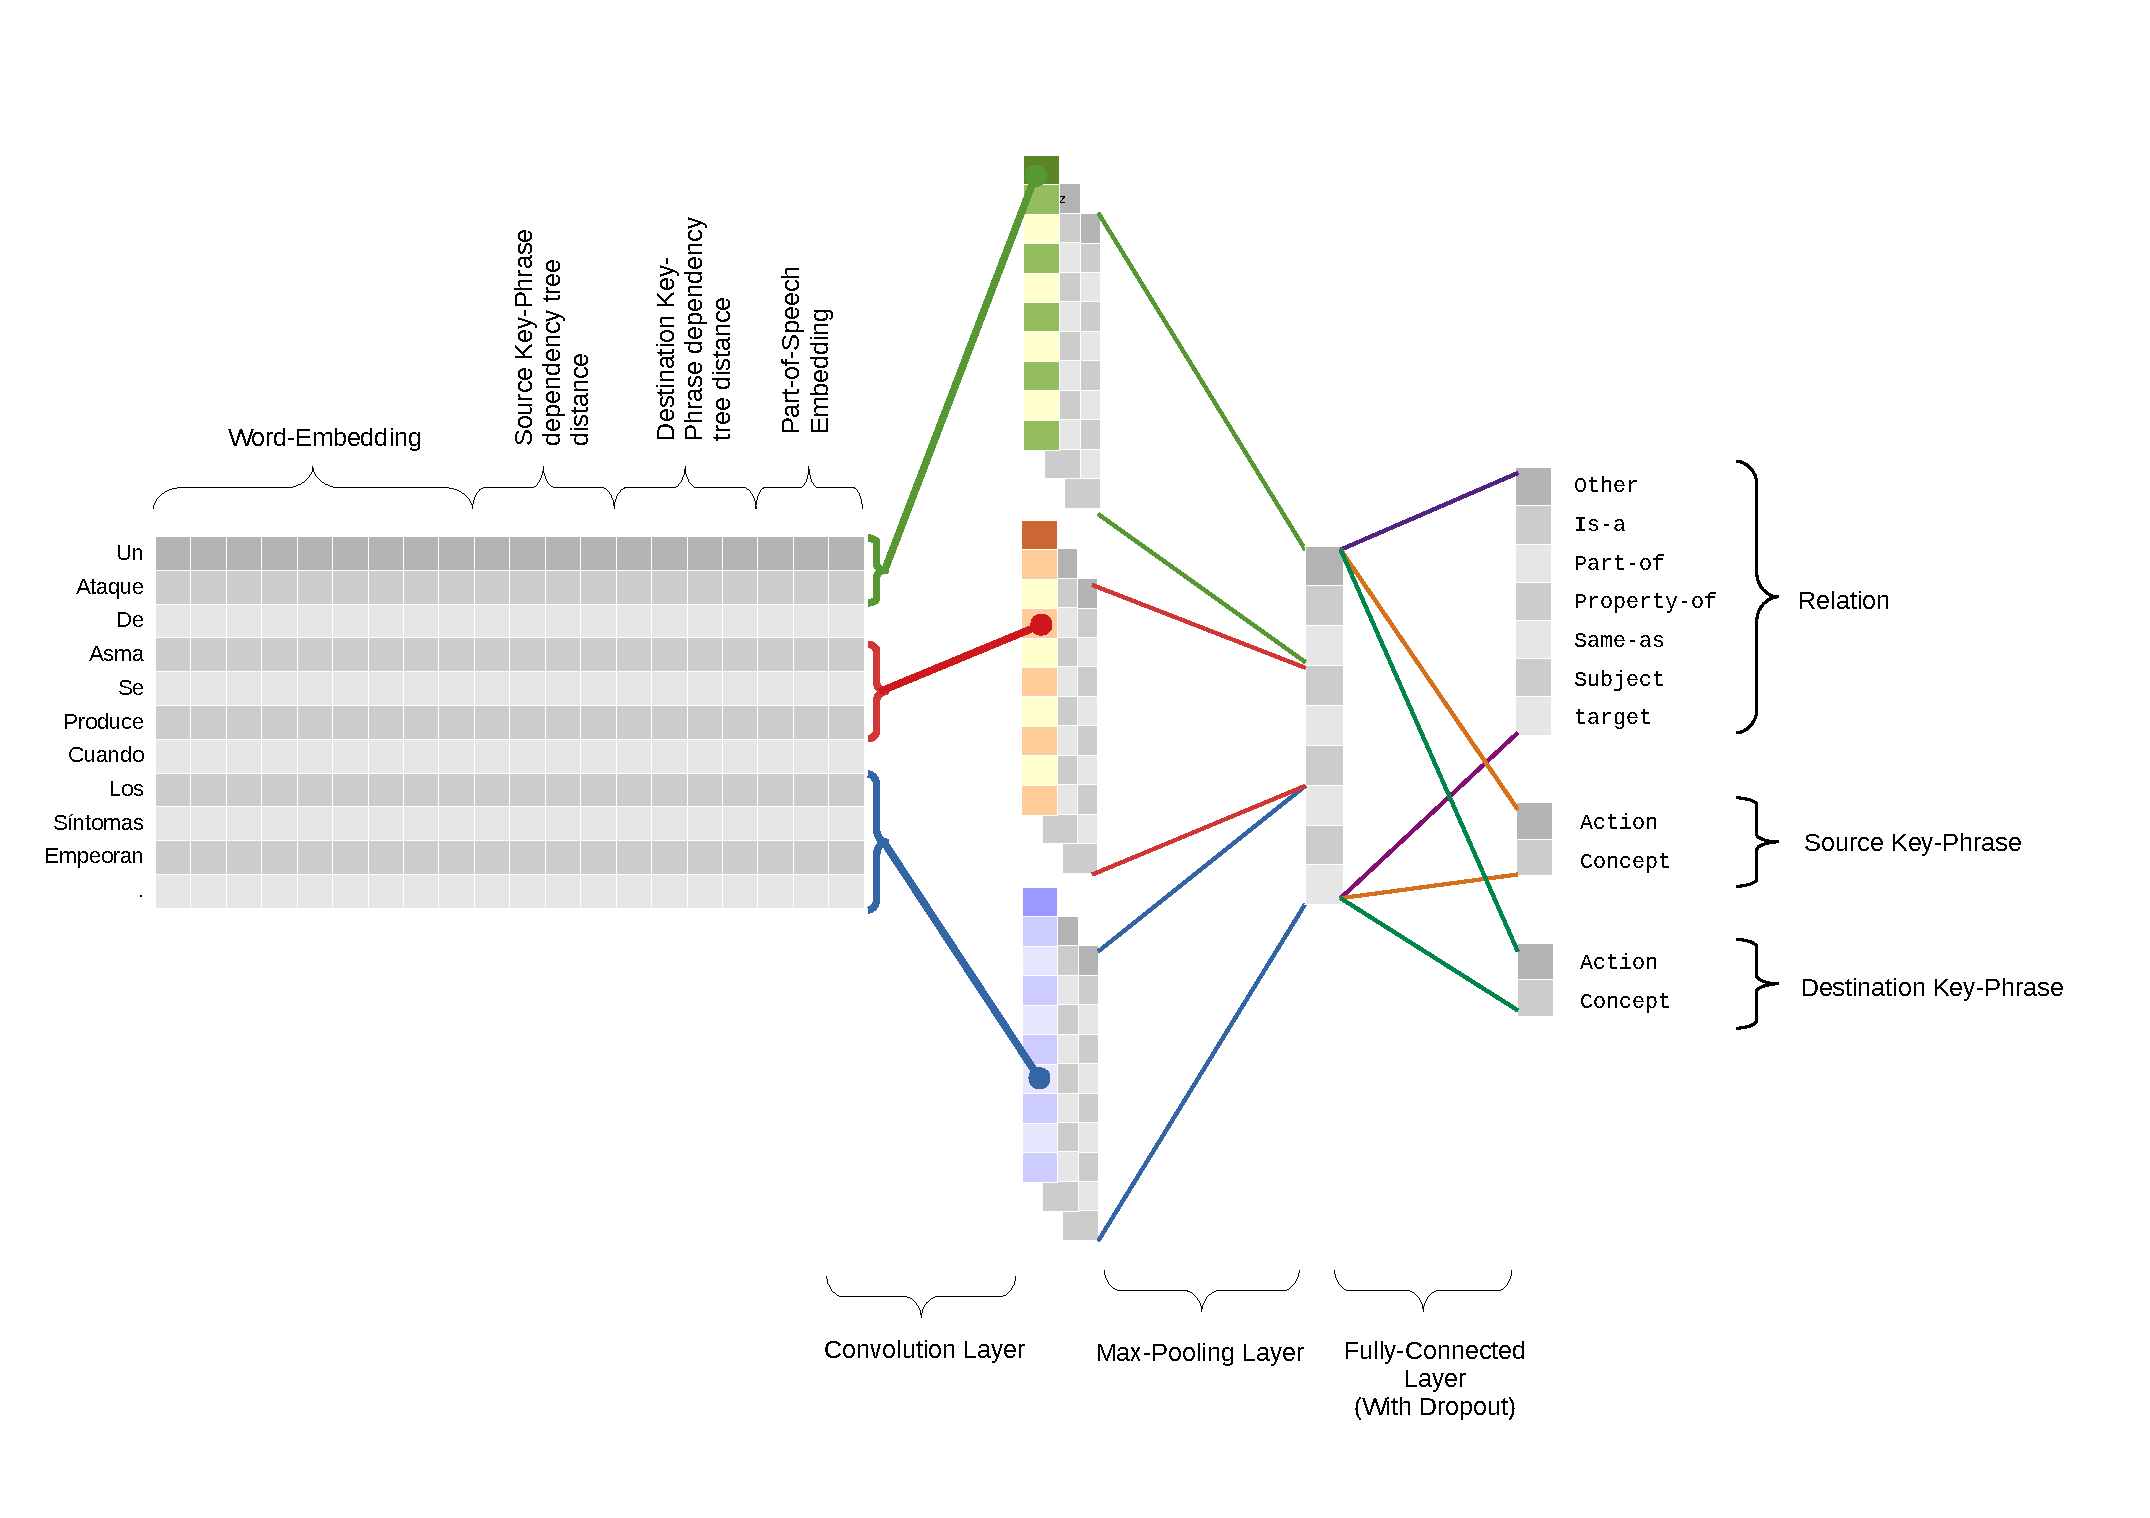
\includegraphics[width=0.9\linewidth,trim={0 1.7cm 0 2.2cm},clip]{diagramtass18.pdf}
    \caption{Layout of the proposed Convolutional Neural Network}
    \label{fig:architecture}
\end{figure}
\end{frame}




%%%%%%%%%%%%%%%%%%%%%%%%%%%%%%%%%%%%%%%%%%%%%%%
%
%   RESULTS
%
%%%%%%%%%%%%%%%%%%%%%%%%%%%%%%%%%%%%%%%%%%%%%%%

\section{Results}


\subsection{Overall Results}

\begin{frame}{Results}
\framesubtitle{Overall Results}
    \begin{table}[ht]
    \centering
\begin{tabular}{r|cccccc|c}
\toprule
% \rotatebox{90}{Scenario} & \rotatebox{90}{plubeda} & \rotatebox{90}{rriveraz} & \rotatebox{90}{upf\_upc} & \rotatebox{90}{TALP} & \rotatebox{90}{VSP} & \rotatebox{90}{baseline} & \rotatebox{90}{Marcelo} \\
{\footnotesize{Scenario}} & {\footnotesize{plubeda}} & {\footnotesize{rriveraz}} & {\footnotesize{upf\_upc}} & {\footnotesize{VSP}} & {\footnotesize{baseline}} & {\footnotesize{Marcelo}} & {\footnotesize{TALP}} \\
\midrule
1 & .71 & \textbf{.744} & .681 & .297 & .566 & .181 & {\footnotesize{N/A*}} \\
2 & .674 & .648 & .622 & .275 & .577 & .255 & \textbf{.722} \\
3 & {\footnotesize{N/A*}} & {\footnotesize{N/A*}} & .036 & .42 & .107 & .018 & \textbf{.448} \\
\bottomrule
avg & .461 & \textbf{.464} & .446 & .331 & .417 & .151 & .39 \\
\end{tabular}
    \caption{Micro-averaged $F1$ score for evaluation scenarios 1 to 3 and global average. \emph{TALP} column shows our model's score. \textbf{N/A*}: Not Available, counted as 0 in the average score.}
    \label{tab:results}
\end{table}
\end{frame}

\subsection{Sub-Task B: Key-Phrase Classification}

\begin{frame}{Results}
\framesubtitle{Sub-Task B: Key-Phrase Classification}
    \begin{table}[t]
 \small
    \centering
\begin{tabular}{r|cc|c}
\toprule
true\textbackslash pred. & Concept &  Action & recall \\
\midrule
Concept &  \textbf{432} &       7 &  .984\\
Action  &   34 &     \textbf{120} & .779\\
\bottomrule
precision & .927 & .945 & $Acc=.931$


\end{tabular}
    \caption{Confusion matrix of our model's predictions for sub-task \emph{B} in scenario 2.}
    \label{tab:confusion2a}
\end{table}
\end{frame}


\subsection{Sub-Task C: Relation Extraction}

\begin{frame}{Results}
\framesubtitle{Sub-Task C: Relation Extraction}
    \begin{table}[ht]
\small
    \centering
    \begin{tabular}{r|ccccccc|c}
\toprule
 true\textbackslash pred. &  \rotatebox{90}{other} &  \rotatebox{90}{is-a} &  \rotatebox{90}{part-of} &  \rotatebox{90}{property-of} &  \rotatebox{90}{same-as} &  \rotatebox{90}{subject} &  \rotatebox{90}{target} & \rotatebox{90}{recall}\\
\midrule
other       &      \textbf{0} &     0 &        0 &            0 &        0 &        0 &       0 & .000 \\
is-a        &     31 &    \textbf{58} &        1 &            2 &        0 &        0 &       0 & .630 \\
part-of     &     26 &     2 &        \textbf{5} &            0 &        0 &        0 &       0 & .152 \\
property-of &     34 &     0 &        3 &           \textbf{18} &        0 &        0 &       3 & .310 \\
same-as     &      0 &     1 &        0 &            0 &        \textbf{0} &        0 &       0 & .000 \\
subject     &     65 &     0 &        0 &            2 &        0 &       \textbf{42} &       8 & .359 \\
target      &     84 &     0 &        1 &            7 &        0 &       12 &      \textbf{91} & .467 \\
\bottomrule
precision & .000 & .951 & .500 & .621 & .000 & .778 & .892 & $F_1=.431$
\end{tabular}
    \caption{Confusion matrix, precision and recall of our model's predictions for sub-task \emph{C} in scenario 2. $F_1$ is micro-averaged for all classes.}
    \label{tab:confusion2b}
\end{table}
    
\end{frame}




%%%%%%%%%%%%%%%%%%%%%%%%%%%%%%%%%%%%%%%%%%%%%%%
%
%   CONCLUSIONS & FUTURE WORK
%
%%%%%%%%%%%%%%%%%%%%%%%%%%%%%%%%%%%%%%%%%%%%%%%

\section{Conclusions}





%%%%%%%%%%%%%%%%%%%%%%%%%%%%%%%%%%%%%%%%%%%%%%%
%
%   CLOSING
%
%%%%%%%%%%%%%%%%%%%%%%%%%%%%%%%%%%%%%%%%%%%%%%%

\begin{frame}[allowframebreaks]{References}

\bibliographystyle{apalike}
\bibliography{bibliography.bib}
\end{frame}

\begin{frame}
\centering
\Huge Thank you for your attention!
\end{frame}


\begin{frame}
\centering
\Huge Questions?
\end{frame}

%%
\end{document}
